% !TEX root = ../intro-stellar-physics.tex

\section{The nucleus}

Experimentally, nuclei are on the order of femtometers\sidenote{Sometimes called a \emph{Fermi}} ($\val{1}{\fermi} = \val{10^{-15}}{\meter}$) in size. Like an atom, the nucleus also has excited states; typical energies for these are on the order of MeV ($\val{1}{\MeV} = \val{10^{6}}{\eV}$). \marginnote{An \newterm{electron volt} (eV) is the energy acquired by an electron being accelerated through a potential difference of 1 volt.} It therefore makes sense to use fm and MeV as our units of length and energy. In these units, the combination
\[	\hbar c = \val{197}{\MeV\,\fermi} \]
to three significant figures. In quantum field theory, the strength of the electromagnetic interaction is characterized by the dimensionless \newterm{fine structure constant}
\[	\alphaF = \frac{e^{2}}{4\pi\epsilon_{0}\hbar c} = \frac{1}{137}, \]
again to three significant figures. From these two quantities, we find the electron (or proton) charge in these units,
\[
	\frac{e^{2}}{4\pi\epsilon_{0}} = \alphaF\hbar c = \val{1.44}{\MeV\,\fermi}.
\]
Put another way, the potential energy between two protons of charge $e$ separated by $\val{1}{\fermi}$ is $\val{1.44}{\MeV}$.

The strong nuclear force differs from electromagnetism and gravity in several ways. First, the strong nuclear force is short-range: the interaction vanishes for distances $\gtrsim\val{2}{\fermi}$. It is weakly attractive for distances $\val{1}{\fermi}\lesssim r\lesssim\val{2}{\fermi}$ and becomes strongly repulsive at distances $\ll\val{1}{\fermi}$. The potential between the neutron and proton in a deuterium (\hydrogen[2]) nucleus (called a deuteron) therefore looks something like that sketched in Fig.~\ref{f.nuclear-potential}. The deuteron's ground state (black dotted line) is at $E_{\mathrm{d}} = -\val{2.2}{\MeV}$, so the nucleus is weakly bound ($|E_{\mathrm{d}}| \ll |V|$, where $V$ is the depth of the potential well).

\begin{marginfigure}[-8\baselineskip]
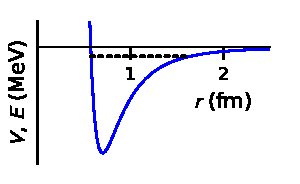
\includegraphics[width=\linewidth]{nuclear-potential}
\caption[Schematic of the nuclear potential]{\label{f.nuclear-potential}Schematic of the nuclear potential for a deuteron (\hydrogen[2]). The binding energy of the deuteron is shown as a black dotted line.}
\end{marginfigure}

\begin{exercisebox}[Depth of nuclear well]
We can estimate the depth of the well in Fig.~\ref{f.nuclear-potential}. Since this is a two-body problem, transfer to center-of-mass coordinates and treat this as a single particle with a reduced mass $m_{p}m_{n}/(m_{p}+m_{n}) \approx m_{n}/2$. Use the uncertainty principle, with $\Delta x$ being the width of the well, to get an estimate of $p\sim\Delta p$ and from this estimate the kinetic energy of the particle. Finally, use the small value of the binding energy (sum of potential and kinetic energies) to estimate the depth of the potential well.
\end{exercisebox}

Also unlike electromagnetism and gravity, the strong nuclear force does not obey superposition: we cannot write the energy of the nucleus as a sum over the potential between all pairs of nucleons. Moreover, the strong nuclear force is not a central force, meaning that it depends on more than just the distance between any two nucleons. The behavior of an atomic nucleus is thus much more complicated to describe than the electronic structure of the atom.

\newthought{Despite these complications, we can construct a phenomenological formula for the nuclear mass that is reasonably accurate.} Let us write the mass of a nucleus with $A$ nucleons---$Z$ protons and $N=A-Z$ neutrons---as
\[
	M(Z,N) = Zm_{p} + Nm_{n} - B(Z,N)/c^{2},
\]
where $B(Z,N)$ is the \newterm{binding energy}---the amount of energy that must be supplied to the nucleus in order to break it into its constituent protons and neutrons.
Because the nuclear force is weakly attractive for separations $\val{1}{\fermi}\lesssim r\lesssim\val{2}{\fermi}$ and repulsive at shorter distances (Fig.~\ref{f.nuclear-potential}), there is a characteristic spacing between nucleons that is a bit larger than $\val{1}{\fermi}$. In a large nucleus, we therefore expect the nucleons to have a roughly constant density, so that the volume of the nucleus is proportional to $A$; experimentally, the radius of the nucleus is roughly\sidenote{The value of the radius depends on how it is measured; scattering with various light particles (protons, neutrons, alpha, electrons) agree, however, that $r_{A}\propto A^{1/3}$.}
\[
	r_{A} = \valrng{1.1}{1.8}{\fermi}\times A^{1/3}.
\]
Notice that because the nucleon-nucleon potential is short-ranged, nucleons in a large nucleus only interact with their nearest neighbors. Indeed the nucleon-nucleon interaction in similar in form to the potential between molecules in a fluid, such as a water drop. This motivates developing a simple formula that gives a decent approximation for the binding energy. For the first term, we estimate the binding energy of a large nucleus as the binding energy of a single nucleon with its neighbors, multiplied by the number of nucleons. Experimentally, it is found that for large nuclei this is the case: the binding energy per nucleon is roughly constant: we say that the nuclear interaction \newterm{saturates}, so that $B(Z,N) \propto A = (Z+N)$.

\begin{exercisebox}[If the strong force were long-range]
To see how the nuclear force differs from the long-range Coulomb and gravitational force, suppose instead that the nuclear force acted like a super-gravity. Use the results from our constant-density model of a star (eq.~[\ref{e.energy-constant-density-sphere}]) to derive how the binding energy would scale with $A$ in this case.
\end{exercisebox}

It is energetically favorable to have equal numbers of neutrons and protons. We therefore define an asymmetry parameter $\eta \equiv (N-Z)/(N+Z) = 1-2Z/A$, so that $-1\le\eta\le1$. The nuclear contribution to the binding energy is maximized for $\eta = 0$ (equal numbers of protons and neutrons). Because the nuclear force does not distinguish between neutrons and protons, the binding energy is quadratic in $\eta$, so that $B$ doesn't depend on the sign of $\eta$. Thus our first approximation for the binding energy is $B \approx (a_{V} - a_{A}\eta^{2}) A$. Here $a_{V}$ and $a_{A}$ are as-yet-undetermined coefficients.

In a fluid drop there is a correction for the surface tension. Heuristically, we imagine that nuclei in the surface have fewer neighbors and are therefore not as bound. We therefore subtract from our formula a term proportional to the surface area, $\propto r_{A}^{2} \propto A^{2/3}$. The next iteration of our liquid-drop approximation is thus $B \approx (a_{V}- a_{A}\eta^{2})A - a_{S}A^{2/3} $.

Finally, the protons in the nucleus are charged and therefore repel one another. This Coulomb repulsion also reduces the binding energy. We therefore subtract a term $\propto Z^{2}/r_{A}\propto Z^{2}/A^{1/3}$ from our mass formula to obtain
\begin{equation}\label{e.liquid-drop}
B = \left(a_{V} -a_{A}\eta^{2}\right) A -  a_{S}A^{2/3} - a_{C} \frac{Z^{2}}{A^{1/3}}. 
\end{equation}
This is a version of the \newterm{semi-empirical mass formula}, also known as the \newterm{Bethe-Weizs\"acker mass formula}.
The coefficients $a_{V},a_{A},a_{S},a_{C}$ are found by fitting the formula to known nuclear masses\sidenote{This fit should have another term to account for the pairing of neutrons and protons, so that the binding energy is  increased for even $Z$ and $N$. We omit that term here for simplicity.}
for measured nuclear masses (Table~\ref{t.liquid-drop}).
\begin{margintable}
\caption[Liquid-drop coefficients]{\label{t.liquid-drop} Coefficients for hte fit to nuclear masses, (\protect\ref{e.liquid-drop}), in units of MeV.}
\begin{tabular}{rrrr}
$a_V$ & $a_A$ & $a_S$ & $a_C$ \\
\hline
15.5 & 22.7 & 16.6 & 0.71\\
\end{tabular}
\end{margintable}

\begin{exercisebox}[The nuclear landscape]
For a given nuclear mass number $A$, derive an expression for the charge number $Z_{\star}(A)$ that maximizes the binding energy (eq.~[\ref{e.liquid-drop}] with coefficients from Table~\ref{t.liquid-drop}).
\begin{enumerate}
\item Plot the ratio $Z_{\star}/A$ for $4\le A\le 128$. Give a physical explanation for the behavior of $Z_{\star}/A$.
\item Plot the binding energy per nucleon $B/A$ as a function of $Z_{\star}$ and $A$, for $4\le A\le 128$.
\item Find the atomic number $Z$ and atomic mass $A$ of the nucleus with the maximum $B/A$.
\end{enumerate}
\end{exercisebox}

\section{Nuclear reactions}

From mass-energy conservation, the heat evolved during a nuclear reaction equals the change in mass of the reacting system. For example, in the reaction
\[
	\helium[3] + \helium[3] \to \helium + \pt + \pt,
\]
the change in mass is
\begin{eqnarray*}
	\lefteqn{2\left[2m_{p}+m_{n}-B(\helium[3])\right] - \left[2m_{p}+2m_{n}-B(\helium)\right] - 2m_{p}} \\
	&=& B(\helium)-B(\helium[3])\\
	&=& \val{28.296}{\MeV} - \val{7.718}{\MeV}\\ &=& \val{20.578}{\MeV}.
\end{eqnarray*}

\begin{exercisebox}[Heat from hydrogen fusing to helium]
Fusion of hydrogen into helium entails converting 4 hydrogen atoms (including the 4 electrons) into 1 helium atom (2 protons, 2 neutrons, 2 electrons) with $B = \val{28.296}{\MeV}$. What is the heat evolved \emph{per hydrogen atom}? Assume that the sun has been shining with its current luminosity over its life. What mass of hydrogen atoms would need to undergo fusion to supply this energy? How large is this mass relative to the total mass of the sun? 
\end{exercisebox}

\newthought{You might at first think that because the nuclear interaction is short-range, the cross-section is something like $\pi r_{n}^{2}$, where $r_{n}\approx\valrng[--]{1}{2}{\fermi}$.} Things are a bit more subtle, however, and in this section we are going to take the reaction-rate apart to understand how it works. First, the ``size'' of a particle is in general proportional to the ``size'' of the wavefunction, which is set by the uncertainty principle, 
\[\pi\left(\frac{\lambda}{2\pi}\right)^{2} = \pi \left(\frac{\hbar}{p}\right)^{2} = \pi\frac{\hbar^{2}}{2mE}.\]
Notice that if we multiply and divide by $c^{2}$, then we can estimate the area as
\[
	\frac{(\hbar c)^{2}}{m_{p} c^{2}} \frac{1}{E} \sim \val{\sci{4}{4}}{\fermi^{2}} \times \left(\frac{\keV}{E}\right) = \val{400}{\barn}\left(\frac{\keV}{E}\right).
\]	
Here we've introduced a convenient unit for cross-sections, the \newterm{barn}\sidenote{as in hitting the broad side of}, with $\val{1}{\barn} = \val{10^{-28}}{\meter^{2}} = \val{100}{\fermi^{2}}$.

The key point is that the size of the wave packet is $\propto 1/E$, which is in general true. This geometrical size of the wave packet is then multiplied by the probability of the nucleons forming a bound state, so we write the nuclear portion of the cross-section as
\[
	\sigma_{\mathrm{nuclear}}(E) = \frac{S(E)}{E}.
\]
The function $S(E)$ contains the details of the nuclear interaction; in general $S(E)$ must be measured experimentally.

The final part of the cross-section concerns the Coulomb potential.
Because protons repel one another, at large separations the nuclei interact via the Coulomb potential. Consider the case of two nuclei with masses\sidenote{When doing kinematics, we shall make the approximation $m\approx A\mb$.} $A_{1}\mb$ and $A_{2}\mb$. Transform to the center-of-mass frame; the problem then reduces to that of one particle, mass $A\mb = A_{1}A_{2}/(A_{1}+A_{2})\times\mb$, moving in a potential, which at large separations is purely Coulomb,
\[ \frac{Z_{1}Z_{2}e^{2}}{4\pi\epsilon_{0}r} = \val{1.44}{\MeV}\times Z_{1}Z_{2}\left(\frac{\val{1}{\fermi}}{r}\right). \]
Fig.~\ref{f.tunneling} has a schematic of the potential. While at short distances the nuclear interaction forms a deep potential well (blue curve), outside the nucleus the Coulomb potential dominates (red curve).
\begin{marginfigure}
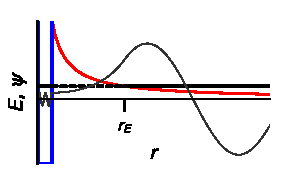
\includegraphics[width=\linewidth]{tunnel-schematic}
\caption{Tunneling through the Coulomb potential barrier. Not to scale.}
\label{f.tunneling}
\end{marginfigure}

\begin{exercisebox}[Turning radius for proton-proton collision in solar plasma]
\label{ex.turning-radius}
For the sun, typical center-of-mass energies are $E \sim \val{1}{\keV}$ (horizontal black line in Fig.~\ref{f.tunneling}). Suppose we have two protons heading towards one another with this kinetic  energy. What is their distance of closest approach?
\end{exercisebox}

As shown in Exercise~\ref{ex.turning-radius}, the turning radius $r_{E}$ at typical stellar energies is much larger than the nuclear radius.  Classically the particle can't penetrate the region $r_{n} < r < r_{E}$ where $E < V$ (dotted black line, Fig.~\ref{f.tunneling}); under classical physics, there would be no nuclear reactions at typical stellar temperatures because two particles would never find themselves close enough to be bound by the nuclear force.

The world is quantum, however, and the uncertainty in a particle's position means there is a small probability for the nucleons to be close enough for the nuclear force to come into play. In the classically forbidden region $r_{n} < r < r_{E}$, the particle wavefunction (thin gray line, Fig.~\ref{f.tunneling}) decreases exponentially, so that the probability to reach $r\sim\val{1}{\fermi}$ is
\[ \mathcal{P}\approx \exp\left[-2\pi^{2}\frac{r_{E}}{\lambda}\right] \]
where $\lambda = h/p$, $p$ being the momentum of the particle.
It is convenient to rewrite the argument of the exponential in terms of the particle energy,
\[ \frac{2\pi^{2}r_{E}}{\lambda} = 2\pi^{2}\left(\frac{Z_{1}Z_{2}e^{2}}{E}\right)
	\left(\frac{p}{h}\right) = \left[\pi \frac{Z_{1}Z_{2}e^{2}\sqrt{2m}}{\hbar}\right]\left(\frac{1}{E}\right)^{1/2}, \]
so that the probability of ``tunneling'' through the Coulomb barrier is
\begin{equation}
\mathcal{P} \approx \exp\left[-\left(\frac{\EG}{E}\right)^{1/2}\right],
\end{equation}
with
\[ \EG \equiv \textrm{``Gamow Energy''} = \left[\frac{2\pi^{2}Z_{1}^{2}Z_{2}^{2}e^{4}m}{\hbar^{2}}\right] = Z_{1}^{2}Z_{2}^{2}A \times \val{979}{\keV}.
\]

Our reaction cross-section is therefore the nuclear cross-section multiplied by the probability of tunneling, 
\begin{equation}\label{e.s-def}
\sigma(E) = \frac{S(E)}{E}\exp\left[-\left(\frac{\EG}{E}\right)\right].
\end{equation}
For many reactions $S(E)$ is nearly constant,
%\sidenote{This is true as long as we are not close to a resonance---an energy level in the compound nucleus that matches the energy of the incoming particle.}
which helps with extrapolating the cross-section from laboratory energies  to the much lower stellar energies.

To get the reaction rate, recall that the mean-free path of a particle is $\ell = (n\sigma)^{-1}$, where $n$ is the density of targets.  For a particle traveling at speed $v$, the mean time between collisions is therefore $\ell/v$; in a large ensemble of particles, this gives the mean rate, $r = n\sigma v$.  Here $v = |\bvec{v}_{1}-\bvec{v}_{2}|$ is the relative velocity between the particles.  

\begin{sidebar}[The thermally averaged cross section]
\label{sb.thermally-averaged-cross-section}
Since the cross-section depends on energy, the rate at which any given particle 1 will react with particles of type 2 having velocities $\bvec{v}_{2}$ in a range $\dif^{3}v_{2}$ is
\[ n_{2} \sigma |\bvec{v}_{1}-\bvec{v}_{2}| \left(\frac{m_{2}}{2\pi kT}\right)^{3/2}\exp\left(-\frac{m_{2}v_{2}^{2}}{2kT}\right) \,\dif^{3}v_{2}. \]
The extra terms are because the particles have a Maxwell-Boltzmann distribution of velocities. To get the total rate per unit volume, we then have to multiply by the number of particles of type 1 having velocities $\bvec{v}_{1}$ in a range $\dif^{3} v_{1}$ and integrate over $\dif^{3}v_{1}\,\dif^{3}v_{2}$:
\begin{eqnarray}\label{e.rate-joint}
\lefteqn{r_{12} = n_{1}n_{2}  \left[\frac{m_{1}m_{2}}{(2\pi kT)^{2}}\right]^{3/2}}
  \nonumber\\ &&\times\int\! \sigma(E) v\exp\left(-\frac{m_{1}v_{1}^{2}}{2kT}-\frac{m_{2}v_{2}^{2}}{2kT}\right)  \,\dif^{3} v_{1}\,\dif^{3}v_{2}.
\end{eqnarray}
Now $E$ and $v$ are the relative energies and velocity in the center-of-mass frame.  We can change variable using the relations
\begin{eqnarray*}
\bvec{v}_{1} &=& \bvec{V} - \frac{m_{2}}{m_{1}+m_{2}} \bvec{v}\\
\bvec{v}_{2} &=& \bvec{V} + \frac{m_{1}}{m_{1}+m_{2}} \bvec{v}.
\end{eqnarray*}
where $V$ is the center-of-mass velocity. It is straightforward to show that $\dif v_{1,x}\,\dif v_{2,x} = \dif V_{x}\dif v_{x}$, and likewise for the $y,z$ directions.  Furthermore, $m_{1}v_{1}^{2} + m_{2}v_{2}^{2} = (m_{1}+m_{2})V^{2} + m v^{2}$, and multiplying and dividing the integral in equation~(\ref{e.rate-joint}) by $m_{1}+m_{2}$ allows us to write
\begin{eqnarray*}
\lefteqn{r_{12} = n_{1}n_{2} \left(\frac{m_{1}+m_{2}}{2kT}\right)^{3/2}\left(\frac{m}{2kT}\right)^{3/2}}\\
&&\times \int\!\dif^{3}V \int\!\dif^{3}v \,\sigma(E)v \exp\left[-\frac{mv^{2}}{2kT}\right]
 \exp\left[-\frac{(m_{1}+m_{2})V^{2}}{2kT}\right].
\end{eqnarray*}
The integral over $\dif^{3}V$ can be factored out and is normalized to unity. Hence we have for the reaction rate between a pair of particles 1 and 2, 
\begin{eqnarray}\label{e.rate}
r_{12} &=& n_{1}n_{2}\left\{\left(\frac{m}{2\pi kT}\right)^{3/2}\int_{0}^{\infty}\! \sigma(E) v \exp\left(-\frac{mv^{2}}{2kT}\right)  4\pi v^{2}\,\dif v\right\}.\nonumber\\
 &\equiv& n_{1}n_{2}\langle\sigma v\rangle.
\end{eqnarray}
The term in $\{\}$ is the averaging over the joint distribution of the cross-section times the velocity, and is usually denoted as $\langle\sigma v\rangle$. Note that if particles 1 and 2 were identical, then we would need to divide $r_{12}$ by 2.

Changing variables to $E = mv^{2}/2$ in equation~(\ref{e.rate}) and inserting the formula for the cross-section, equation~(\ref{e.s-def}), gives
\begin{equation}\label{e.integral}
\langle\sigma v\rangle = \left(\frac{8}{\pi m}\right)^{1/2}\left(\frac{1}{kT}\right)^{3/2}\int_{0}^{\infty}\!S(E)\exp\left[-\left(\frac{\EG}{E}\right)^{1/2}-\frac{E}{kT}\right]\,\dif E.
\end{equation}
Now, we've assumed that $S(E)$ varies slowly; but look at the argument of the exponential. This is a competition between a rapidly rising term $\exp[-(\EG/E)^{1/2}]$ and a rapidly falling term $\exp(-E/kT)$. As a result, the exponential will have a strong peak, and we can expand the integrand in a Taylor series about the maximum. Let 
\[
f(E) = -\left(\frac{\EG}{E}\right)^{1/2} - \frac{E}{kT}.
\]
Then we can write 
\begin{eqnarray*}
\lefteqn{\int_{0}^{\infty}\!S(E)\exp\left[-\left(\frac{\EG}{E}\right)^{1/2}-\frac{E}{kT}\right]\,\dif E}\\
&\approx&
	\int_{0}^{\infty}\! S(\Epk)\exp\left[f(\Epk) + \frac{1}{2}\left.\frac{\dif^{2} f}{\dif E^{2}}\right|_{E=\Epk}\left(E-\Epk\right)^{2}\right].
\end{eqnarray*}
Here $\Epk$ is found by solving $(\dif f/\dif E)|_{E=\Epk} = 0$. This trick allows us to turn the integral into a Gaussian!

Solving for \Epk, we get
\[
\Epk = \frac{\EG^{1/3}(kT)^{2/3}}{2^{2/3}},
\]
and 
\[ \exp\left[f(\Epk)\right] = \exp\left[-3\left(\frac{\EG}{4kT}\right)^{1/3}\right].
\]
Further,
\[
\left.\frac{1}{2}\frac{\dif^{2}f}{\dif E^{2}}\right|_{E=\Epk} = -\frac{3}{2(2\EG)^{1/3}(kT)^{5/3}} = -\frac{3}{4\Epk kT}.
\]
Defining a variable $\Delta = 4(\Epk kT/3)^{1/2}$, our integral becomes
\begin{eqnarray}\label{e.integral2}
\lefteqn{\langle\sigma v\rangle = \left(\frac{8}{\pi m}\right)^{1/2}\left(\frac{1}{kT}\right)^{3/2} S(\Epk)} \nonumber\\
&&\times 
  \exp\left[-3\left(\frac{\EG}{4kT}\right)^{1/3}\right]\int_{0}^{\infty}\!\exp\left[-\frac{(E-\Epk)^{2}}{(\Delta/2)^{2}}\right]\,\dif E.
\end{eqnarray}
%How well does this approximation do?  Figure~\ref{f.integrand} shows the integrand (\emph{solid line}) and the approximation by a Gaussian (\emph{dashed line}).  Although the integrand is skewed to the right, the area is approximately the same.
Another simplification can be made because both the Gaussian and the original integrand go to zero as $E\to 0$.  As a result, we can extend the lower bound of our integral (eq.~[\ref{e.integral2}]) to $-\infty$, and obtain
\begin{eqnarray}\label{e.rate2}
\langle\sigma v\rangle &\approx& \left(\frac{8}{\pi m}\right)^{1/2}\left(\frac{1}{kT}\right)^{3/2} S(\Epk) \exp\left[-3\left(\frac{\EG}{4kT}\right)^{1/3}\right]\frac{\Delta}{2}\nonumber\\
 &=& \frac{2^{13/6}}{\sqrt{3m}}\frac{\EG^{1/6}}{(kT)^{2/3}} \exp\left[-3\left(\frac{\EG}{4kT}\right)^{1/3}\right]  S(\Epk).
\end{eqnarray}
\end{sidebar}

%\begin{marginfigure}
%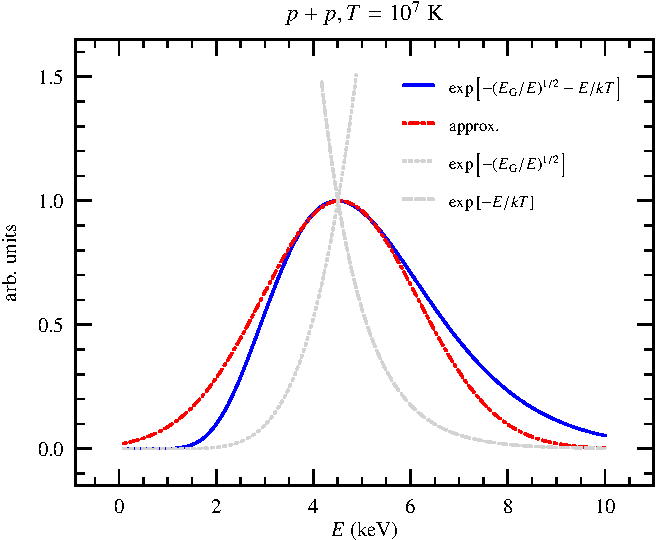
\includegraphics[width=\linewidth]{coulomb_integrand}
%\caption[Terms in integrand for calculating Coulomb barrier]{Integrand of eq.~(\protect\ref{e.integral}) (\emph{solid line}) and the Gaussian (\emph{dot-dashed line}) constructed by expanding to second order the argument of the exponential. The parameters for $\EG$ were taken from the $p+p$ reactions ($Z_{1}Z_{2}=1$, $A = 1/2$), and the temperature is $\val{10^{7}}{\K}$.  Note that the grey curves, showing the two terms of the exponential, have been rescaled to fit on the same plot.}
%\label{f.integrand}
%\end{marginfigure}

At stellar energies, the reaction rates are incredibly sensitive to temperature. To quantify this, approximate the rate at a given temperature as a power-law, $r(T)\propto T^{n}$. Then the exponent is
\begin{equation}\label{e.exponent}
 n(T) = \dd{\ln r}{\ln T} = -\frac{2}{3} + \left(\frac{\EG}{4kT}\right)^{1/3},
\end{equation}
as you can verify for yourself (Exercise~\ref{ex.power-law}). On to some numbers. Table~\ref{t.reaction} lists quantities for some common reactions. 
In the table, the exponent $n(T)$ is evaluated at $T = \val{10^{7}}{\K}$. Note the large value of $n(T)$ at stellar temperatures. 
 
\begin{table}[hb]
\caption{\label{t.reaction} Parameters for non-resonant reactions}
\begin{tabular}{lrrrrrr}
 & $\pt+\pt$ & $\pt+\helium[3]$ & $\helium[3]+\helium[3]$ & $\pt+\lithium[7]$ & $\pt+\carbon$\\
\hline
%$A$ & 1/2 & 3/4 & 3/2 & 0.88 & 0.92 \\
%$Z_{1}Z_{2}$ & 1 & 2 & 4 & 3 & 6 \\
$\EG$ (MeV) & 0.489 & $2.94$ & $23.5$ & $7.70$ & $32.5$\\
%$\EG/(4k)$ (GK) & $1.4$ & $8.5$ & $68.0$ & $22.0$ & $94.0$ \\
$\Epk|_{T=\val{10^{7}}{\K}}$ (keV) & 4.5 & 8.2 & 16.3 & 11.3 & 18.2\\
%$\Delta/\Epk|_{T=\val{10^{7}}{\K}}$ & 1.0 & 0.75 & 0.53 & 0.64 & 0.50 \\
$n(T = \val{10^{7}}{\K})$ & 4.6 & 8.8 & 18.3 & 12.4 & 20.5\\
\end{tabular}
\end{table}

\begin{exercisebox}[Approximating a function as a power-law]
\label{ex.power-law}
Suppose we wish to approximate a function $f(x)$ at a point $x_{0}$ with a power-law, $p(x;A,n) = Ax^{n}$. Impose the condition $p(x_{0};A,n) = f(x_{0})$ and $\dif p/\dif x |_{x=x_{0}} = \dif f/\dif x|_{x=x_{0}}$ to find the parameters $A$ and $n$, and show that
\[
	n = \DD{\ln f}{\ln x}.
\]
Apply this to the reaction rate, eq.~(\ref{e.rate2}), and thus derive eq.~(\ref{e.exponent}).
\end{exercisebox}

